\section{Teilaufgabe 13}
\begin{aufgabe}
    Lesen Sie aus dem Bode-Diagramm des offenen Regelkreises die 
    Stabilitätsreserve (für die 2 Fälle $K_p < \frac{1}{K_g}$ und 
    $K_p > \frac{1}{K_g}$ ).
\end{aufgabe}
\[ K_P \cdot K_g < 1 \]
\begin{figure}[h!]
    \centering
    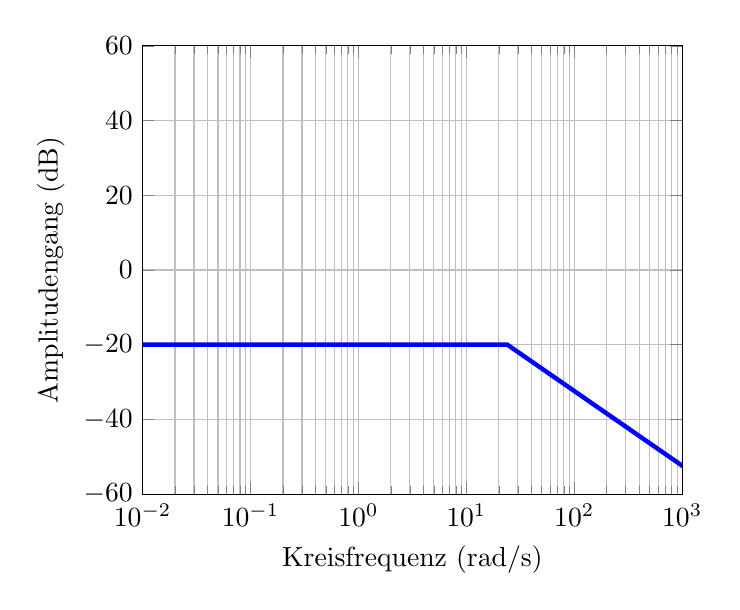
\begin{tikzpicture}[scale=1]
        \begin{semilogxaxis}
            [xmin=1e-2, 
                xmax=1e3, 
                ymin=-60, 
                ymax=60, 
                ytick={-60, -40, ..., 60}, 
                xlabel=Kreisfrequenz (rad/s),
                ylabel=Amplitudengang (dB),
                grid=both]
            \addplot[mark=none, color=blue, ultra thick] coordinates 
                {(0.002398,-20) 
                (23.98,-20) 
                (2398,-60)};
        \end{semilogxaxis}
    \end{tikzpicture}
    \\
    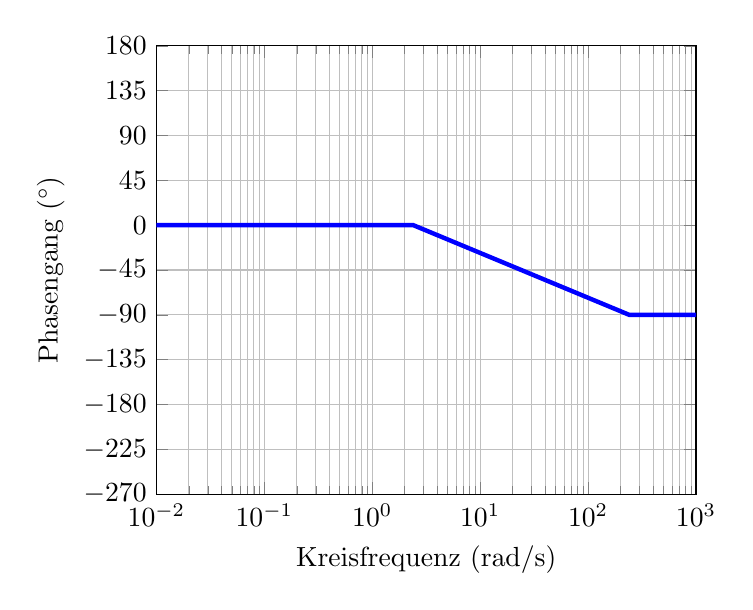
\begin{tikzpicture}[scale=1]
        \begin{semilogxaxis}
            [xmin=1e-2, 
                xmax=1e3, 
                ymin=-270, 
                ymax=180, 
                ytick={-270, -225, ..., 180}, 
                xlabel=Kreisfrequenz (rad/s),
                ylabel=Phasengang ($^\circ$),
                grid=both]
            \addplot[mark=none, color=blue, ultra thick] coordinates 
                {(0.002398,0) 
                (2.398,0) 
                (239.8,-90) 
                (2398,-90)};
        \end{semilogxaxis}
    \end{tikzpicture}
\end{figure}
\[ \varphi_r = \infty \qquad A_r = \infty \]
\clearpage
\[ K_P \cdot K_g > 1 \]
\begin{figure}[h!]
    \centering
    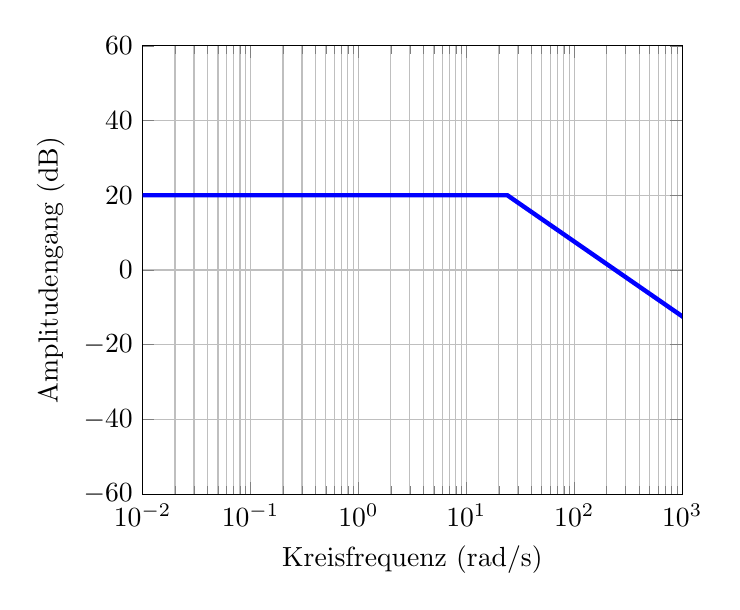
\begin{tikzpicture}[scale=1]
        \begin{semilogxaxis}
            [xmin=1e-2, 
                xmax=1e3, 
                ymin=-60, 
                ymax=60, 
                ytick={-60, -40, ..., 60}, 
                xlabel=Kreisfrequenz (rad/s),
                ylabel=Amplitudengang (dB),
                grid=both]
            \addplot[mark=none, color=blue, ultra thick] coordinates 
                {(0.002398,20) 
                (23.98,20) 
                (2398,-20)};
        \end{semilogxaxis}
    \end{tikzpicture}
    \\
    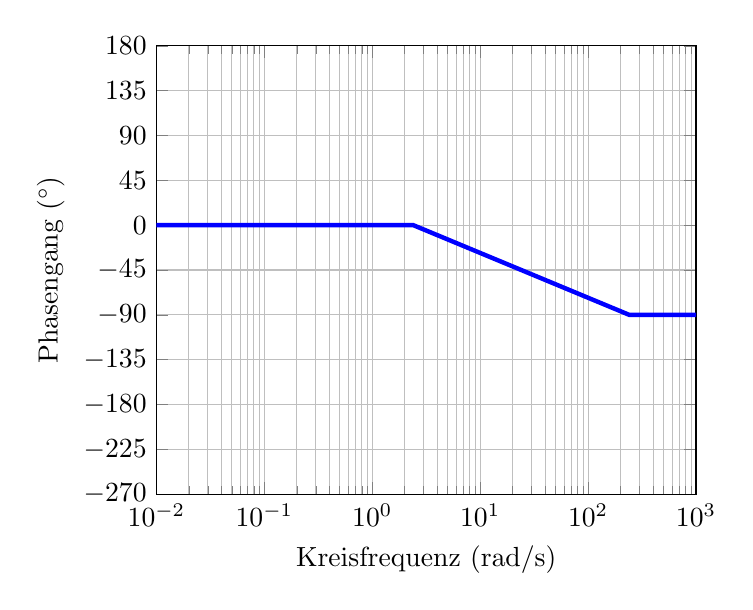
\begin{tikzpicture}[scale=1]
        \begin{semilogxaxis}
            [xmin=1e-2, 
                xmax=1e3, 
                ymin=-270, 
                ymax=180, 
                ytick={-270, -225, ..., 180}, 
                xlabel=Kreisfrequenz (rad/s),
                ylabel=Phasengang ($^\circ$),
                grid=both]
            \addplot[mark=none, color=blue, ultra thick] coordinates 
                {(0.002398,0) 
                (2.398,0) 
                (239.8,-90) 
                (2398,-90)};
        \end{semilogxaxis}
    \end{tikzpicture}
\end{figure}
\[ \varphi_r = 90 \ldots 180^\circ \qquad A_r = \infty \]
